%
% Copyright 2018 Joel Feldman, Andrew Rechnitzer and Elyse Yeager.
% This work is licensed under a Creative Commons Attribution-NonCommercial-ShareAlike 4.0 International License.
% https://creativecommons.org/licenses/by-nc-sa/4.0/
%
\graphicspath{{./figures/basic/}}

\chapter{The Basics}
\label{chap basics}
We won't make this section of the text too long --- all we really want to do
here is to take a short memory-jogging excursion through little bits and
pieces you should remember about sets and numbers. The material in this chapter will not
be (directly) examined.


\section{Numbers}
Before we do anything else, it is very important that we agree on the definitions
and names of some important collections of numbers.

\begin{itemize}
\item Natural numbers --- These are the ``whole numbers'' 1,2,3,\dots that we
learn first at about the same time as we learn the alphabet. We will denote this
collection of numbers by the symbol ``$\mathbb{N}$''. The symbol $\mathbb{N}$ is
written in a type of bold-face font that we call ``black-board bold'' (and is
definitely \emph{not} the same symbol as $N$). You should become used to
writing a few letters in this way since it is typically used to denote
collections of important numbers.
Unfortunately there is often some confusion as to whether or not zero should be
included\footnote{This lack of agreement comes from some debate over how
``natural'' zero is --- ``how can nothing be something?'' It was certainly not
used by the ancient Greeks who really first looked at proof and number.
If you are a mathematician then generally $0$ is not a natural number. If you
are a computer scientist then $0$ generally is.}. In this text
the natural numbers does not include zero.

Notice that the set of natural numbers is \emph{closed} under addition and
multiplication. This means that if you take any two natural numbers and
add them you get another natural number. Similarly if you take any two natural
numbers and multiply them you get another natural number. However the set is not
closed under subtraction or division; we need negative numbers and fractions to
make collections of numbers closed under subtraction and division.

Two important subsets of natural numbers are:
\begin{itemize}
 \item Prime numbers --- a natural number is prime when the only natural
numbers that divide it exactly are 1 and itself. Equivalently it cannot be
written as the product of two natural numbers neither of which are 1. Note that
1 is not a prime number\footnote{If you let 1 be a prime number then you have
to treat $1\times2\times 3$ and $2\times 3$ as different factorisations of the
number 6. This causes headaches for mathematicians, so they don't let 1 be
prime.}.

\item Composite numbers --- a natural number is a composite number when it is
not prime.
\end{itemize}
Hence the number $7$ is prime, but $6 = 3\times 2$ is composite.

\item Integers --- all positive and negative numbers together with the number
zero. We denote the collection of all integers by the symbol ``$\mathbb{Z}$''.
Again, note that this is not the same symbol as ``$Z$'', and we must write it in
the same black-board bold font. The $\mathbb{Z}$ stands for the German
\emph{Zahlen} meaning numbers\footnote{Some schools (and even some provinces!!) may use
``$I$'' for integers, but this is extremely non-standard and they really should
use correct notation.}. Note that $\mathbb{Z}$ is closed under addition,
subtraction and multiplication, but not division.

Two important subsets of integers are:
\begin{itemize}
 \item Even numbers --- an integer is even if it is exactly divisible by $2$, or
equivalently if it can be written as the product of 2 and another integer. This
means that $-14, 6$ and $0$ are all even.
\item Odd numbers --- an integer is odd when it is not even. Equivalently it
can be written as $2k+1$ where $k$ is another integer. Thus $11 = 2\times 5+1$
and $-7 = 2\times(-4)+1$ are both odd.
\end{itemize}

\item Rational numbers --- this is all numbers that can be written
as the ratio of two integers. That is, any rational number $r$ can be written
as $p/q$ where $p,q$ are integers. We denote this collection by $\mathbb{Q}$
standing for \emph{quoziente} which is Italian for quotient or ratio. Now we
finally have a set of numbers which is closed under addition, subtraction,
multiplication and division (of course you still need to be careful not to
divide by zero).

\item Real numbers --- generally we think of these numbers as numbers that can
be written as decimal expansions and we denote it by $\mathbb{R}$. It is beyond the
scope of this text to go into the details of how to give a precise definition of real
numbers, and the notion that a real number can be written as a decimal
expansion will be sufficient.

It took mathematicians quite a long time to realise that there were numbers
that could not be written as ratios of integers\footnote{The existence of such
numbers caused mathematicians (particularly the ancient Greeks) all sorts of
philosophical problems. They thought that the natural numbers were somehow
fundamental and beautiful and ``natural''. The rational numbers you can get very
easily by taking ``ratios'' --- a process that is still somehow quite sensible.
There were quite influential philosophers (in Greece at least) called
Pythagoreans (disciples of Pythagoras originally) who saw numbers as almost
mystical objects explaining all the phenomena in the universe, including beauty
--- famously they found fractions in musical notes etc and ``numbers constitute
the entire heavens''. They believed that everything could be explained by whole
numbers and their ratios. But soon after Pythagoras' theorem was discovered, so
were numbers that are not rational. The first proof of the existence of
irrational numbers is sometimes attributed to Hippasus in around 400BCE (not
really known). It seems that his philosopher ``friends'' were not very happy
about this and essentially exiled him. Some accounts suggest that he was drowned
by them. }. The first numbers that were shown to be not-rational are
square-roots of prime numbers, like $\sqrt{2}$. Other well known examples are
$\pi$ and $e$. Usually the fact that some numbers cannot be represented as
ratios of integers is harmless because those numbers can be approximated by
rational numbers to any desired precision.

The reason that we can approximate real numbers in this way is the
surprising fact that between any two real numbers, one can always find a
rational number. So if we are interested in a particular real number we can
always find a rational number that is extremely close. Mathematicians refer
to this property by saying that $\mathbb{Q}$ is \emph{dense} in $\mathbb{R}$.
\end{itemize}
So to summarise
\begin{defn}[Sets of numbers]
  This is not really a definition, but you should know these symbols
 \begin{itemize}
  \item $\mathbb{N} = $ the natural numbers,
  \item $\mathbb{Z} = $ the integers,
  \item $\mathbb{Q} = $ the rationals, and
  \item $\mathbb{R} = $ the reals.
 \end{itemize}

\end{defn}



\subsection*{More on Real Numbers}
In the preceding paragraphs we have talked about the decimal expansions of real
numbers and there is just one more point that we wish to touch on. The decimal
expansions of rational numbers are always \emph{periodic}, that is the expansion
eventually starts to repeat itself. For example
\begin{align*}
  \frac{2}{15} &= 0.133333333\dots \\
  \frac{5}{17} &=
0.\underline{
2941176470588235}2941176470588235\underline{2941176470588235}
294117647058823\dots
\end{align*}
where we have underlined some of the last example to make the period clearer.
On the other hand, irrational numbers, such as $\sqrt{2}$ and $\pi$, have
expansions that never repeat.

If we want to think of real numbers as their decimal expansions, then we need
those expansions to be unique. That is, we don't want to be able to write down
two different expansions, each giving the same real number. Unfortunately there
are an infinite set of numbers that do not have unique expansions. Consider the
number 1. We usually just write ``1'', but as a decimal expansion it is
\begin{align*}
  1.00000000000\dots
\end{align*}
that is, a single 1 followed by an infinite string of 0's. Now consider the
following number
\begin{align*}
  0.99999999999\dots
\end{align*}
This second decimal expansions actually represents the same number ---
the number $1$. Let's prove this. First call the real number this
represents $q$, then
\begin{align*}
  q &=0.99999999999\dots
\end{align*}
Let's use a little trick to get rid of the long string of trailing 9's. Consider
$10q$:
\begin{align*}
  q &=0.99999999999\dots\\
  10q &=9.99999999999\dots
\end{align*}
If we now subtract one from the other we get
\begin{align*}
  9q &= 9.0000000000\dots
\end{align*}
and so we are left with $q=1.0000000\dots$. So both expansions represent the
same real number.

Thankfully this sort of thing only happens with rational numbers of a
particular form --- those whose denominators are products of 2s and 5s. For
example
\begin{align*}
  \frac{3}{25} &= 1.200000\dots = 1.19999999\dots\\
  -\frac{7}{32} &= -0.2187500000\dots = -0.2187499999\dots\\
  \frac{9}{20} &= 0.45000000\dots = 0.4499999\dots
\end{align*}
We can formalise this result in the following theorem (which we haven't proved
in general, but it's beyond the scope of the text to do so):
\begin{theorem}
 Let $x$ be a real number. Then $x$ must fall into one of the following two
categories,
\begin{itemize}
 \item $x$ has a unique decimal expansion, or
 \item $x$ is a rational number of the form $\frac{a}{2^k 5^\ell}$ where $a\in
\mathbb{Z}$ and $k,l$ are non-negative integers.
\end{itemize}
In the second case, $x$ has exactly two expansions, one that ends in an
infinite string of 9's and the other ending in an infinite string of 0's.
\end{theorem}
When we do have a choice of two expansions, it is usual to avoid the one that
ends in an infinite string of 9's and write the other instead (omitting the
infinite trailing string of 0's).

\section{Sets}\label{sec sets}
All of you will have done some basic bits of set-theory in school. Sets,
intersection, unions, Venn diagrams etc etc. Set theory now appears so
thoroughly throughout mathematics that it is difficult to imagine how
Mathematics could have existed without it. It is really quite surprising that
set theory is a much newer part of mathematics than calculus. Mathematically rigorous set
theory was really only developed in the 19th Century --- primarily by Georg
Cantor\footnote{An extremely interesting mathematician who is responsible for
much of our understanding of infinity. Arguably his most famous results are
that there are more real numbers than integers, and that there are an infinite
number of different infinities. His work, though now considered to be extremely
important, was not accepted by his peers, and he was labelled ``a corrupter of
youth'' for teaching it. For some reason we know that he spent much of his
honeymoon talking and doing mathematics with Richard Dedekind.}. Mathematicians
were using sets before then (of course), however they were doing so without
defining things too rigorously and formally.

In mathematics (and elsewhere, including ``real life'') we are used to dealing
with collections of things. For example
\begin{itemize}
\item a family is a collection of relatives.
\item hockey team is a collection of hockey players.
\item shopping list is a collection of items we need to buy.
\end{itemize}

Generally when we give mathematical definitions we try to make them very
formal and rigorous so that they are as clear as possible. We need to do this
so that when we come across a mathematical object we can decide with complete
certainty whether or not it satisfies the definition.

Unfortunately, it is the case that giving a completely rigorous definition of
``set'' would take up far more of our time than we would really
like\footnote{The interested reader is invited to google (or whichever
search engine you prefer --- DuckDuckGo?) ``Russell's paradox'', ``Axiomatic set theory''
and ``Zermelo-Fraenkel set theory'' for a more complete and \emph{far} more
detailed discussion of the basics of sets and why, when you dig into them a
little, they are not so basic.}.

\begin{defn}[A not-so-formal definition of set]
 A ``set'' is a collection of distinct objects. The objects are referred to as
``elements'' or ``members'' of the set.
\end{defn}

Now --- just a moment to describe some conventions. There are many of these in
mathematics. These are not firm mathematical rules, but just traditions. It
makes it much easier for people reading your work to understand what you are
trying to say.
\begin{itemize}
\item Use capital letters to denote sets, $A,B, C, X, Y$ etc.
\item Use lower case letters to denote elements of the sets $a,b,c,x,y$.
\end{itemize}
So when you are writing up homework, or just describing what you are
doing, then if you stick with these conventions people reading your work
(including the person marking your exams) will know --- ``Oh $A$ is that set
they are talking about'' and ``$a$ is an element of that set.''. On the other
hand, if you use any old letter or symbol it is correct, but confusing for the
reader. Think of it as being a bit like spelling --- if you don't spell words
correctly people can usually still understand what you mean, but it is much easier if
you spell words the same way as everyone else.

We will encounter more of these conventions as we go --- another good one is
\begin{itemize}
\item The letters $i,j,k,l,m,n$ usually denote integers (like
$1,2,3,-5,18,\dots$).
\item The letters $x,y,z,w$ usually denote real numbers (like $1.4323, \pi,
\sqrt{2}, 6.0221415\times 10^{23} \dots$ and so forth).
\end{itemize}

So now that we have defined sets, what can we do with them? There is only thing
we can ask of a set
\begin{quote}
``Is this object in the set?''
\end{quote}
and the set will answer
\begin{quote}
  ``yes'' or ``no''
\end{quote}
For example, if $A$ is the set of even numbers we can ask ``Is 4 in $A$?'' We
get back the answer ``yes''. We write this as
\begin{align*}
  4 \in A
\end{align*}
While if we ask  ``Is $3$ in $A$?'', we get back the answer ``no''.
Mathematically we would write this as
\begin{align*}
  3 \notin A
\end{align*}
So this symbol ``$\in$'' is mathematical shorthand for ``is an element of'',
while the same symbol with a stroke through it ``$\notin$'' is shorthand for
``is not an element of''.

Notice that both of these statements, though they are written down as short
strings of three symbols, are really complete sentences. That is, when we
read them out we have
\begin{align*}
  \text{``$4 \in A$''}
  &&& \text{is read as} && \text{``Four is an element of  $A$.''} \\
  \text{``$3 \notin A$''}
  &&& \text{is read as} &&  \text{``Three is not an element of $A$.''}
\end{align*}
The mathematical symbols like ``$+$'', ``$=$'' and ``$\in$'' are
shorthand\footnote{Precise definitions aside, by ``shorthand'' we mean a
collection of accepted symbols and abbreviations to allow us to write more
quickly and hopefully more clearly. People have been using various systems of
shorthand as long as people have been writing. Many of these are used and
understood only by the individual, but if you want people to be able to
understand what you have written, then you need to use shorthand that
is commonly understood.} and mathematical statements like ``$4+3=7$'' are complete
sentences.


This is an important point --- mathematical writing is just like any other sort
of writing. It is very easy to put a bunch of symbols or words down on the
page, but if we would like it to be easy to read and understand, then we have
to work a bit harder. When you write mathematics you should keep in mind that
someone else should be able to read it and understand it.
\begin{quote}
 \emph{Easy reading is damn hard writing.}
\end{quote}
\begin{flushright}
 Nathaniel Hawthorne, but possibly also a few others like Richard
Sheridan.
\end{flushright}


We will come across quite a few different sets when doing
mathematics. It must be completely clear from the definition how
to answer the question ``Is this object in the set or not?''
\begin{itemize}
\item ``Let $A$ be the set of even integers between 1 and 13.'' --- nice and
clear.
\item ``Let $B$ be the set of tall people in this class room.'' --- not clear.
\end{itemize}
More generally if there are only a small number of elements in the set we just
list them all out
\begin{itemize}
\item ``Let $C = \{1,2,3\}$.''
\end{itemize}
When we write out the list we put the elements inside braces ``$\{ \cdot \}$''.
Note that the order we write things in doesn't matter
\begin{align*}
  C & = \{1,2,3\} = \{2,1,3\} = \{3,2,1\}
\end{align*}
because the only thing we can ask is ``Is this object an element of $C$?'' We
cannot ask more complex questions like ``What is the third element of $C$?'' ---
we require more sophisticated mathematical objects to ask such
questions\footnote{The interested reader is invited to look at ``lists'',
``multisets'', ``totally ordered sets'' and ``partially ordered sets''
amongst many other mathematical objects that generalise the basic idea of
sets.}. Similarly, it doesn't matter how many times we write the same object in
the list
\begin{align*}
  C &= \{1,1,1,2,3,3,3,3,1,2,1,2,1,3\} = \{1,2,3\}
\end{align*}
because all we ask is ``Is $1 \in C$?''. Not ``how many times is 1 in $C$?''.

Now --- if the set is a bit bigger then we might write something like this
\begin{itemize}
\item $C = \{1,2,3,\dots,40\}$ the set of all integers between 1 and 40
(inclusive).
\item $A = \{1,4,9,16,\dots\}$ the set of all perfect squares\footnote{i.e. 
integers that can be written as the square of another integer.}
\end{itemize}
The ``$\dots$'' is again shorthand for the missing entries. You have to be
careful with this as you can easily confuse the reader
\begin{itemize}
\item $B = \{3,5,7,\dots\}$ --- is this all odd primes, or all odd numbers
bigger than 1 or ?? What is written is not sufficient for us to have a firm
idea of what the writer intended.
\end{itemize}
Only use this where it is completely clear by context. A few extra words can
save the reader (and yourself) a lot of confusion.
\begin{quote}
 \emph{Always think about the reader.}
\end{quote}
% \begin{flushright}
%  The authors.
% \end{flushright}



\section{Other Important Sets}
We have seen a few important sets above --- namely $\mathbb{N}, \mathbb{Z},
\mathbb{Q}$ and $\mathbb{R}$. However, arguably the most important set in
mathematics is the empty set.
\begin{defn}[Empty set]
  The empty set (or null set or void set) is the set which contains no
elements. It is denoted $\es$. For any object $x$, we always
have $x \notin \es$; hence $\es = \{ \}$.
\end{defn}
Note that it is important to realise that the empty set is not \emph{nothing}; think of it
as an empty bag. Also note that with quite a bit of hard work you can actually define the
natural numbers in terms of the empty set. Doing so is very formal and well beyond the
scope of this text.

% \begin{eg}[sets containing the empty set] \textbf{DELETE ME}\\
%  With that in mind, consider
% the following examples:
% \begin{itemize}
% \item $A = \{1,2,\es\}$ --- this set contains three elements; the numbers one
% and two and the empty set. Note --- it is okay for a set to contain other sets.
% \item $B = \{\es\}$ --- this set is not the empty set --- it contains a single
% element, being the empty set. Remember the bag analogy: this is a bag that
% contains an empty bag.
% \item $C = \{\es, \{\es\} \}$ --- this set contains two elements; the empty set
% and the set that contains the empty set (our set $B$ above).
% \end{itemize}
% \end{eg}

When a set does not contain too many elements it is fine to specify it by listing out its
elements.  But for infinite sets or even just big sets we can't do this and instead we
have to give the defining rule. For example the set of all perfect square numbers we
write as
\begin{align*}
  S &= \{x \st x = k^2 \mbox{ where } k \in \mathbb{Z} \}
\end{align*}
Notice we have used another piece of shorthand here, namely $\st$, which
stands for ``such that'' or ``so that''. We read the above statement as ``$S$ is
the set of elements $x$ such that $x$ equals $k$-squared where $k$ is an
integer''. This is the standard way of writing a set defined by a rule, though there are
several shorthands for ``such that''. We shall use two them:
\begin{align*}
  P &= \{ p \st p \mbox{ is prime} \} = \{ p \,|\, p \mbox{ is prime} \}
\end{align*}
Other people also use ``:'' as shorthand for ``such that''. You should 
recognise all three of these shorthands.

\begin{eg}[examples of sets]
  Even more examples\dots
\begin{itemize}
 \item Let $A = \{2,3,5,7,11,13,17,19\}$ and let
 \begin{align*}
  B &= \{ a \in A | a<8\} = \{2,3,5,7\}
  \end{align*}
  the set of elements of $A$ that are strictly less than 8.

\item Even and odd integers
\begin{align*}
E &= \{ n | n \mbox{ is an even integer} \} \\
 &= \{n | n =2k \mbox{ for some $k \in \mathbb{Z}$} \} \\
 &= \{2n | n \in \mathbb{Z}\},
\end{align*}
and similarly
\begin{align*}
  O &= \{ n | n \mbox{ is an odd integer} \} \\
  &= \{2n+1 | n \in \mathbb{Z}\}.
\end{align*}

\item Square integers
\begin{align*}
  S &= \{n^2 | n \in \mathbb{Z}\}.
\end{align*}
The set\footnote{Notice here we are using another common piece of mathematical
short-hand. Very often in mathematics we will be talking or writing about some
object, like the set $S$ above, and then we will create a closely related
object. Rather than calling this new object by a new symbol (we could have used
$T$ or $R$ or\dots), we instead use the same symbol but with some sort of accent
--- such as the little single quote mark we added to the symbol $S$ to make
$S'$ (read ``S prime''). The point of this is to let the reader know that this
new object is related to the original one, but not the same. You might also see
$\dot{S}, \hat{S}, \bar{S}, \tilde{S}$ and others.} $S'= \set{n^2 | n \in
\mathbb{N}}$ is not the same as $S$ because $S'$ does not contain the number
$0$, which is definitely a square integer and $0$ is in $S$. We could also write
$S = \set{n^2 | n \in \mathbb{Z}, n \geq 0}$ and $S=\set{n^2 | n=0,1,2,\dots}$.
\end{itemize}
\end{eg}


The sets $A$ and $B$ in the above example illustrate an important point. Every
element in $B$ is an element in $A$, and so we say that $B$ is a subset of $A$
\begin{defn}
Let $A$ and $B$ be sets. We say ``$A$ is a subset of $B$'' if every
element of $A$ is also an element of $B$. We denote this $A \subseteq B$ (or $B
\supseteq A$). If $A$ is a subset of $B$ and $A$ and $B$ are not the same , so
that there is some element of $B$ that is not in $A$ then we say that $A$ is a
proper subset of $B$. We denote this by $A \subset B$ (or $B \supset A$).
\end{defn}
Two things to note about subsets:
\begin{itemize}
\item Let $A$ be a set. It is always the case that $\es \subseteq A$.
\item If $A$ is not a subset of $B$ then we write $A \not\subseteq B$. This is
the same as saying that there is some element of $A$ that is not in $B$. That
is, there is some $a \in A$ such that $a \notin B$.
\end{itemize}
\begin{eg}[subsets]
Let $S = \{1,2\}$. What are all the subsets of $S$? Well --- each element of
$S$ can either be in the subset or not (independent of the other elements of
the set). So we have $2\times2 = 4$ possibilities: neither $1$ nor $2$ is in the
subset, $1$ is but $2$ is not, $2$ is but $1$ is not, and both $1$ and $2$ are.
That is
\begin{align*}
  \es, \{1\}, \{2\}, \{1,2\} & \subseteq S
\end{align*}
This argument can be generalised with a little work to show that a set that
contains exactly $n$ elements has exactly $2^n$ subsets.
\end{eg}

In much of our work with functions later in the text we will need to work with
subsets of real numbers, particularly segments of the ``real line''. A
convenient and standard way of representing such subsets is with interval
notation.
\begin{defn}[Open and closed intervals of $\mathbb{R}$] \label{def intervals}
  Let $a, b \in \mathbb{R}$ such that $a<b$. We name the subset of all
numbers between $a$ and $b$ in different ways depending on whether or not the
ends of the interval ($a$ and $b$) are elements of the subset.
  \begin{itemize}
   \item The closed interval $[a,b] = \{x \in \mathbb{R} : a \leq x \leq b\}$
--- both end points are included.
   \item The open interval $(a,b) = \{x \in \mathbb{R} : a < x < b\}$ ---
neither end point is included.
  \end{itemize}

  We also define half-open\protect\footnote{Also called ``half-closed''. The
preference
for one term over the other may be related to whether a 500ml glass containing
250ml of water is half-full or half-empty.} intervals which contain one
end point but not the other:
  \begin{align*}
  (a,b] &= \{ x \in \mathbb{R} : a < x \leq b\}
  & [a,b) &= \{ x \in \mathbb{R} : a \leq x < b\}
  \end{align*}
  We sometimes also need unbounded intervals
  \begin{align*}
  [a, \infty) &= \{ x \in \mathbb{R} : a \leq x \}
  & (a, \infty) &= \{ x \in \mathbb{R} : a < x \} \\
  (\infty, b] &= \{ x \in \mathbb{R} : x \leq b \}
  & (\infty, b) &= \{ x \in \mathbb{R} : x < b \}
  \end{align*}
  These unbounded intervals do not include ``$\infty$'', so that end of the
interval is always open\footnote{Infinity is
not a real number. As mentioned in an earlier footnote, Cantor proved that
there are an infinite number of different infinities and so it is incorrect
to think of $\infty$ as being a single number. As such it cannot be an element
in an interval of the real line. We suggest that the reader that wants to learn
more about how mathematics handles infinity look up transfinite numbers and
transfinite arithmetic. Needless to say these topics are beyond the scope of
this text.}.
\end{defn}


\subsection*{More on Sets}
So we now know how to say that one set is contained within another. We will now
define some other operations on sets. Let us also start to be a bit more precise
with our definitions and set them out carefully as we get deeper into the
text.
\begin{defn}
 Let $A$ and $B$ be sets. We define the union of $A$ and $B$, denoted $A \cup
B$, to be the set of all elements that are in at least one of $A$ or $B$.
\begin{align*}
  A \cup B &= \{x | x\in A \mbox{ or } x \in B \}
\end{align*}
\end{defn}
It is important to realise that we are using the word ``or'' in a careful
mathematical sense. We mean that $x$ belongs to $A$ or $x$ belongs to $B$
\emph{or both}. Whereas in normal every-day English ``or'' is often used to be
``exclusive or'' --- $A$ or $B$ but not both\footnote{When you are asked for
your dining preferences on a long flight you are usually asked something
like ``Chicken or beef?'' --- you get one or the other, but not both. Unless
you are way at the back near the toilets in which case you will be presented
with which ever meal was less popular. Probably fish.}.

We also start the definition by announcing ``Definition''
so that the reader knows ``We are about to define something important''. We
should also make sure that everything is (reasonably) self-contained --- we are
not assuming the reader already knows $A$ and $B$ are sets.

It is vital that we make our definitions clear otherwise anything we do with the
definitions will be very difficult to follow. As writers we must try to be nice
to our readers\footnote{If you are finding this text difficult to follow then
please complain to us authors and we will do our best to improve it.}.

\begin{defn}
 Let $A$ and $B$ be sets. We define the intersection of $A$ and $B$, denoted $A
\cap B$, to be the set of elements that belong to both $A$ and $B$.
\begin{align*}
 A \cap B &= \{ x \;|\; x\in A \mbox{ and } x \in B \}
\end{align*}
\end{defn}
Again note that we are using the word ``and'' in a careful mathematical sense
(which is pretty close to the usual use in English).

\begin{eg}[Union and intersection]
Let $A = \{1,2,3,4 \}$, $B = \{p : p \mbox{ is prime} \}$,
$C = \{5,7,9\}$ and $D = \{\mbox{even positive integers}\}$. Then
\begin{align*}
  A \cap B &= \{2,3\} \\
  B \cap D &= \{2 \} \\
  A \cup C &= \{1,2,3,4,5,7,9\} \\
  A \cap C &= \es
\end{align*}
In this last case we see that the two sets have no elements in common --- they
are said to be~\emph{disjoint}.
\end{eg}

\section{Functions}
Now that we have reviewed basic ideas about sets we can start doing more
interesting things with them --- functions.

When we are introduced to functions in mathematics, it is almost always as
formulas. We take a number $x$ and do some things to it to get a new number
$y$. For example,
\begin{align*}
  y = f(x) &= 3x-7
\end{align*}
Here, we take a number $x$, multiply it by 3 and then subtract seven to get the
result.

This view of functions --- a function is a formula --- was how mathematicians
defined them up until the 19th century. As basic ideas of sets became better
defined, people revised ideas surrounding functions. The more modern definition of a
function between two sets is that it is a rule which assigns to each element of the first
set a unique element of the second set.

Consider the set of days of the week, and the set containing the alphabet
\begin{align*}
  A &= \set{\text{Sunday, Monday, Tuesday, Wednesday, Thursday, Friday,
Saturday, Sunday}}\\
  B &= \set{\text{a,b,c,d,e,\dots,x,y,z}}
\end{align*}
We can define a function $f$ that takes a day (that is, an element of $A$) and
turns it into the first letter of that day (that is, an element of $B$). This
is a valid function, though there is no formula. We can draw a picture
of the function as
\begin{fig}
\begin{center}
 \includegraphics[height=4cm]{days}
\end{center}
\end{fig}
Clearly such pictures will work for small sets, but will get very messy for
big ones. When we shift back to talking about functions on real numbers, then we
will switch to using graphs of functions on the Cartesian plane.

This example is pretty simple, but this serves to illustrate some important
points. If our function gives us a rule for taking elements in $A$ and turning
them into elements from $B$ then
\begin{itemize}
 \item the function must be defined for all elements of $A$ --- that is, no
matter which element of $A$ we choose, the function must be able to give us an
answer. Every function must have this property.
 \item on the other hand, we don't have to ``hit'' every element from $B$. In
the above example, we miss almost all the letters in $B$. A function that does
reach every element of $B$ is said to be ``surjective'' or ``onto''.
\item a given element of $B$ may be reached by more than one element of $A$. In
the above example, the days ``Tuesday'' and ``Thursday'' both map to the
letter $T$ and similarly the letters $S$ is mapped to by both
``Sunday'' and ``Saturday''. A function which does not do this, that is, every
element in $A$ maps to a different element in $B$ is called ``injective'' or
``one-to-one'' --- again we will come back to this later when we discuss inverse function
in Section~\ref{sec inverse functions}.
\end{itemize}

Summarising this more formally, we have
\begin{defn}
\label{def function}
 Let $A, B$ be non-empty sets. A function $f$ from $A$ to $B$, is a rule or
formula that takes elements of $A$ as inputs and returns elements of $B$ as
outputs. We write this as
\begin{align*}
  f: A \to B
\end{align*}
and if $f$ takes $a \in A$ as an input and returns $b\in B$ then we write this
as $f(a) = b$. Every function must satisfy the following two conditions
\begin{itemize}
\item The function must be defined on every possible input from the set $A$.
That is, no matter which element $a \in A$ we choose, the function must return
an element $b \in B$ so that $f(a)=b$.

\item The function is only allowed to return one result for each
input\footnote{You may have learned this in the context of plotting functions on
the Cartesian plane, as ``the vertical line test''. If the graph intersects a
vertical line twice, then the same $x$-value will give two $y$-values and so
the graph does not represent a function.}. So if we find that $f(a)=b_1$ and
$f(a)=b_2$ then the only way that $f$ can be a function is if $b_1$ is exactly
the same as $b_2$.
\end{itemize}
\end{defn}
We must include the input and output sets $A$ and $B$ in the definition of the
function. This is one of the reasons that we should not think of
functions as just formulas. The input and output sets have proper mathematical
names, which we give below:
\begin{defn}
Let $f:A \to B$ be a function. Then
\begin{itemize}
\item the set $A$ of inputs to our function is the ``domain'' of $f$,
\item the set $B$ which contains all the results is called the codomain,
\item We read ``$f(a) = b$'' as ``$f$ of $a$ is $b$'', but sometimes we might
say ``$f$ maps $a$ to $b$'' or ``$b$ is the image of $a$''.

\item The codomain must contain all the possible results of the function, but
it might also contain a few other elements. The subset of $B$ that is
exactly the outputs of $A$ is called the ``range'' of $f$. We define it more
formally by
\begin{align*}
	\text{range of } f &= \set{b \in B \;|\; \text{there is some } a \in
A \text{ so that } f(a) = b} \\
  &= \set{f(a) \in B \;|\; a \in A}
\end{align*}
  The only elements allowed in that set are those elements of $B$ that are the
images of elements in $A$.
\end{itemize}
\end{defn}


\begin{eg}[domains and ranges]
Let us go back to the ``days of the week'' function example that we
worked on above, we can define the domain, codomain and range:
\begin{itemize}
 \item The domain, $A$, is the set of days of the week.
\item The codomain, $B$, is the 26 letters of the alphabet.
\item The range is the set $\set{F,M,T,S,W}$ --- no other elements of $B$ are
images of inputs from $A$.
\end{itemize}
\end{eg}
\begin{eg}[more domains and ranges]
A more numerical example --- let $g: \mathbb{R} \to \mathbb{R}$ be defined
by the formula $g(x) = x^2$. Then
\begin{itemize}
 \item the domain and codomain are both the set of all real numbers, but
 \item the range is the set $[0, \infty)$.
\end{itemize}

Now --- let $h:[0,\infty) \to [0,\infty)$ be defined by the formula $h(x) =
\sqrt{x}$. Then
\begin{itemize}
 \item the domain and codomain are both the set $[0,\infty)$, that is all
non-negative real numbers, and
 \item in this case the range is equal to the codomain, namely $[0, \infty)$.
\end{itemize}
\end{eg}
\begin{eg}[piece-wise function]
\label{eg piecewise}
Yet another numerical example.
\begin{align*}
  V:[-1,1] \to \mathbb{R} && \text{defined by }
  V(t) &= \begin{cases}
          0 & \text{if } -1 \leq t < 0 \\
	  120 & \text{if } 0 \leq t \leq 1
          \end{cases}
\end{align*}
  This is an example of a ``piece-wise'' function --- that is, one that is not
defined by a single formula, but instead defined piece-by-piece. This function
has domain $[-1,1]$ and its range is $\set{0,120}$. We could interpret this
function as measuring the voltage across a switch that is flipped on at time $t=0$.
\end{eg}

Almost all the functions we look at from here on will be formulas. However it
is important to note, that we have to include the domain and codomain when we
describe the function. If the domain and codomain are not stated explicitly then
we should assume that both are $\mathbb{R}$.


\begin{comment}
\subsection*{Injections, Surjections and Inverses}
\textbf{I agree --- let us leave this until we review graphing functions, makes
discussions of inverses much easier.}

Given a function $f: A \to B$, that takes elements of $A$ and maps them to
elements of $B$, we might\footnote{Really there is no ``might'' about it, we
will ask this about lots of important functions we meet later in the text.} ask
--- is there another function $g: B \to A$ that undoes whatever it was that $f$
did to take things back to where we started.

More precisely, if we have a function $f: A \to B$, we would like to find the
``inverse'' function, denoted $f^{-1}:B \to A$ so that
\begin{align*}
  f^{-1}( f(a) ) &= a.
\end{align*}
Let us read this last statement carefully. Start with $a \in A$ and ``do'' $f$
to it to get an element $b\in B$. So we know $b = f(a)$. We need our new
``inverse'' function to take $b$ as an input, undo what $f$ did and return $a$.
That is
\begin{align*}
  f^{-1}(b) = f^{-1}(\;\underbrace{f(a)}_{=b}\;) = a
\end{align*}
It is not immediately obvious when such an inverse function should exist, and
for many functions it does not.
\begin{eg}
Above we looked at the function
\begin{align*}
  g : \mathbb{R} \mapsto \mathbb{R} && \text{defined by } g(x) &= x^2
\end{align*}
We'd like to look for an inverse function --- temporarily call it $h$. To
try to build it, let's first experiment a little with $g$\dots
\begin{align*}
  g(0) &= 0 \\
  g(1) &= 1 \\
  g(2) &= 4
\end{align*}
So if $h$ undoes $g$ we would need
\begin{align*}
  h(0) &= 0 \\
  h(1) &= 1 \\
  h(4) &= 2
\end{align*}
This seems okay so far, but we also have
\begin{align*}
  g(-1) &= 1 & g(-2) &= 4
\end{align*}
 So we would need
\begin{align*}
  h(1) &= -1 & h(4)=-2
\end{align*}
But this means that $h$ cannot be a function, because for the same input, $4$,
it would have to give two different outputs, $-2$ and $+2$. So for this
function, no inverse function exists.
\end{eg}


\textbf{A couple more pages of stuff here.}
\end{comment}

\section{Parsing Formulas}
\label{sec parsing}
Consider the formula
\begin{align*}
  f(x) &= \frac{1+x}{1+2x-x^2}
\end{align*}
  This is an example of a simple rational function --- that is, the ratio of
two polynomials. When we start to examine these functions later in the text, it
is important that we are able to understand how to evaluate such functions at
different values of $x$. For example
\begin{align*}
  f(5) &= \frac{1+5}{1+10-25} = \frac{6}{-14} = -\frac{3}{7}
\end{align*}
More important, however, is that we understand how we decompose this function
into simpler pieces. Since much of your calculus course will involve creating and
studying complicated functions by building them up from simple pieces, it is important
that you really understand this point.


Now to get there we will take a small excursion into what are called
parse-trees. You already implicitly use these when you evaluate the function at
a particular value of $x$, but our aim here is to formalise this
process a little more.

We can express the steps used to evaluate the above formula as a tree-like
diagram\footnote{Such trees appear in many areas of mathematics and computer science. The
reason for the name is that they look rather like trees --- starting from their base they
grow and branch out towards their many leaves. For some reason, which remains mysterious,
they are usually drawn upside down.}.
We can decompose this formula as the following tree-like diagram
\begin{fig}
\label{fig tree rational}
  \begin{center}
  \includegraphics[height=7cm]{tree1}

  A parse tree of the function $\frac{1+x}{1+2x-x^2}$.
  \end{center}
\end{fig}
Let us explain the pieces here.
\begin{itemize}
 \item The picture consists of boxes and arrows which are called ``nodes'' and
``edges'' respectively.
 \item There are two types of boxes, those containing numbers and the variable
$x$, and those containing arithmetic operations ``$+$'',``$-$'',
``$\times$'' and ``$/$''.
 \item If we wish to represent the formula $3+5$, then we can draw this as the
following cherry-like configuration
\begin{nfig}
  \begin{center}
   \includegraphics[width=2cm]{cherry1}
  \end{center}
\end{nfig}
 which tells us to take the numbers ``$3$'' and ``$5$'' and add them together
to get $8$.
\begin{nfig}
\begin{center}
  \begin{tabular}{m{2cm} c m{2cm}}
 \includegraphics[width=2cm]{cherry1}
  & \text{ evaluates to } &
  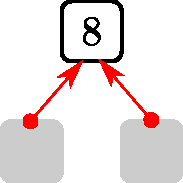
\includegraphics[width=2cm]{cherry1a}
  \end{tabular}
\end{center}
\end{nfig}
  \item By stringing such little ``cherries'' together we can describe more
complicated formulas. For example, if we compute ``$(3+5)\times 2$'', we first
compute ``$(3+5)$'' and then multiply the result by 2. The corresponding
diagrams are
\end{itemize}
\begin{wfig}
\begin{center}
  \begin{tabular}{m{3cm} c m{3cm} c m{3cm}}
 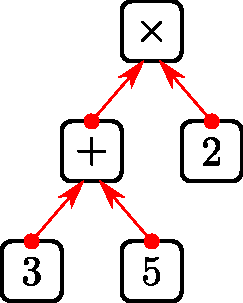
\includegraphics[width=3cm]{cherry2}
  & \text{ evaluates to }
  & 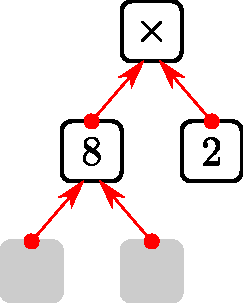
\includegraphics[width=3cm]{cherry2a}
  & \text{ evaluates to }
  & 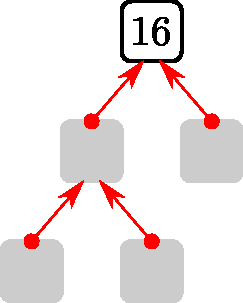
\includegraphics[width=3cm]{cherry2b}
  \end{tabular}
\end{center}
\end{wfig}

The tree we drew in Figure~\ref{fig tree rational} above representing our formula has $x$
in some of the boxes,
and so when we want to compute the function at a particular value of $x$ --- say
at $x=5$ --- then we replace those ``$x$''s in the tree by that value and then
compute back up the tree. See the example below
\begin{fig}
\begin{center}
\begin{tabular}{c m{55mm} c m{55mm} c}
  Start
  & \includegraphics[width=50mm]{tree1b}
  & $\mapsto$
  & 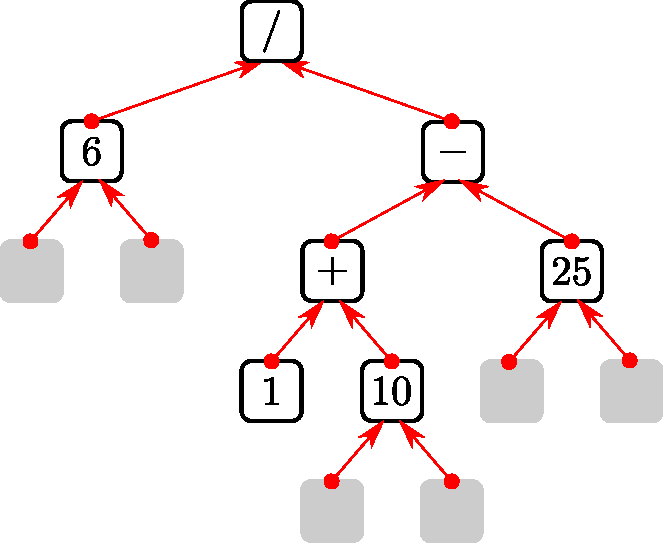
\includegraphics[width=50mm]{tree1b2}
  &
  \\[15ex]
  $\mapsto$
  & 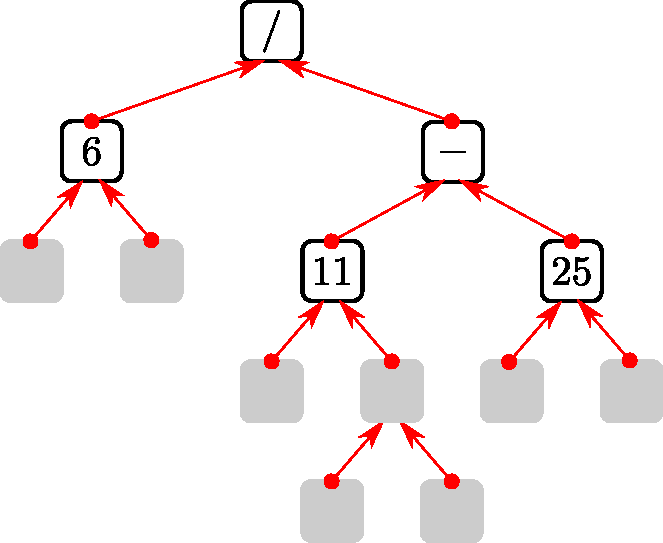
\includegraphics[width=50mm]{tree1b3}
  & $\mapsto$
  & 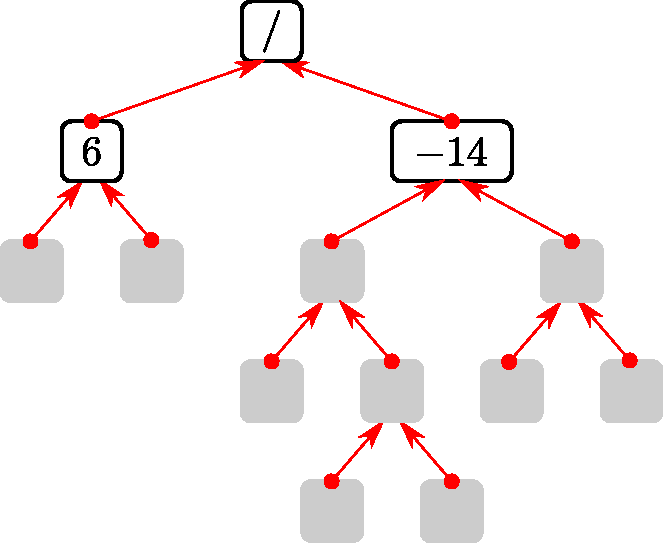
\includegraphics[width=50mm]{tree1b4}
  & \\[15ex]
  $\mapsto$
  & 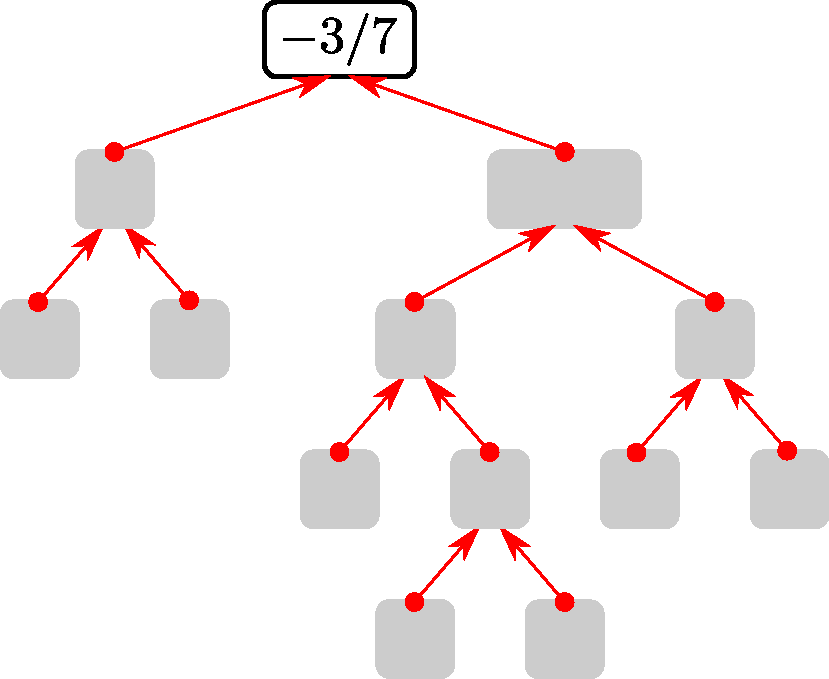
\includegraphics[width=50mm]{tree1b5}
  & & and we are done.
\end{tabular}
\end{center}
\end{fig}

This is not the only parse tree associated with the formula for $f(x)$; we
could also decompose it as
\begin{fig}
\begin{center}
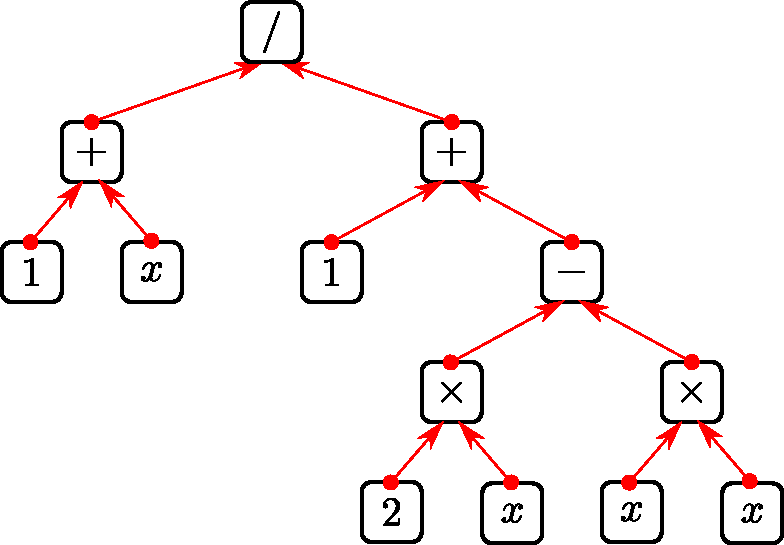
\includegraphics[height=5cm]{tree1a}
\end{center}
\end{fig}
We are able to do this because when we compute the denominator $1+2x-x^2$, we
can compute it as
\begin{align*}
  1+2x-x^2 &= \text{ either } (1+2x)-x^2 \text{ or } = 1 + (2x-x^2).
\end{align*}
Both\footnote{We could also use, for example, $1+2x-x^2 = (1-x^2)+2x$.} are
correct because addition is ``associative''. Namely
\begin{align*}
  a+b+c &= (a+b)+c = a+(b+c).
\end{align*}
Multiplication is also associative:
\begin{align*}
  a \times b \times c &= (a \times b) \times c = a \times (b \times c).
\end{align*}

\begin{eg}[parsing a formula]
Consider the formula
  \begin{align*}
  g(t) &= \left(\frac{t+\pi}{t-\pi} \right) \cdot \sin\left( \frac{t+\pi}{2}
\right).
\end{align*}
  This introduces a new idea --- we have to evaluate $\frac{t+\pi}{2}$ and then
compute the sine of that number. The corresponding tree can be written as
\begin{efig}
\begin{center}
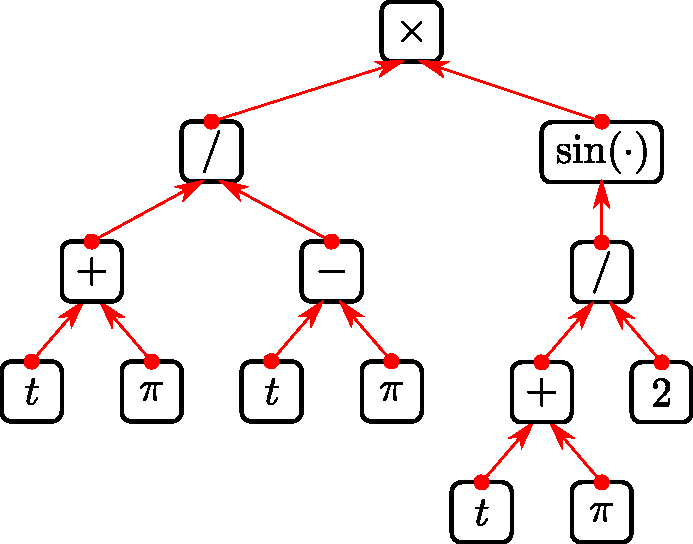
\includegraphics[height=5cm]{tree2}
\end{center}
\end{efig}
  If we want to evaluate this at $t = \pi/2$ then we get the following\dots
\begin{wfig}
\begin{center}
\begin{tabular}{c m{58mm} c m{58mm} c}
  Start
  & 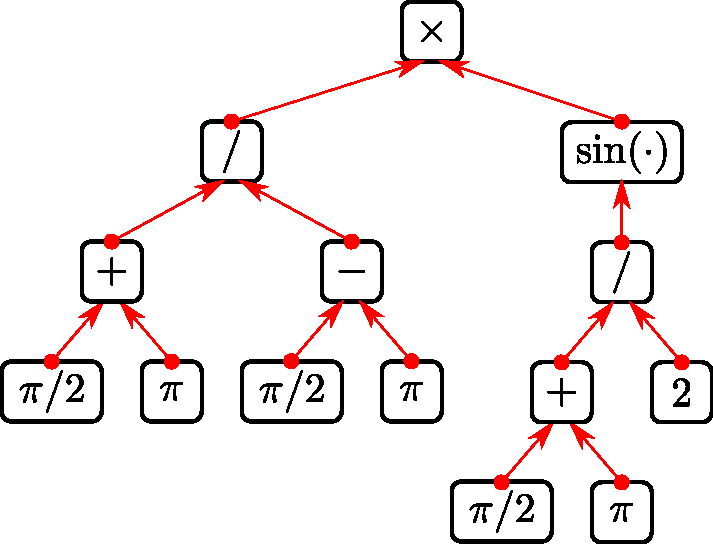
\includegraphics[width=55mm]{tree2a}
  & $\mapsto$
  & 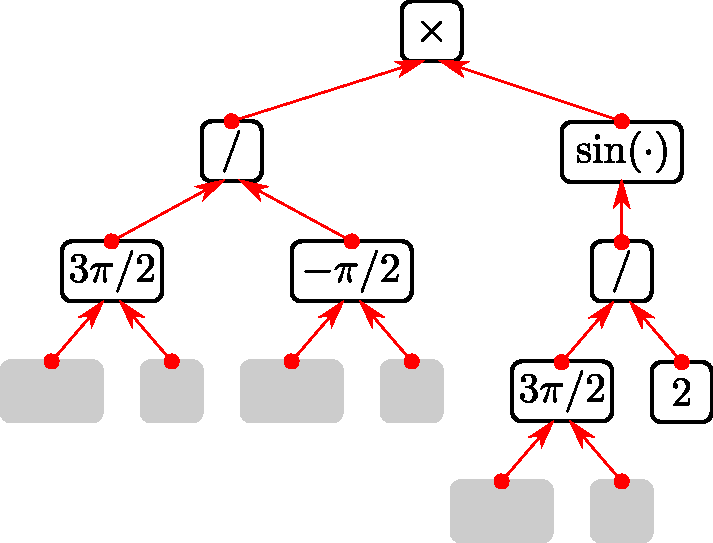
\includegraphics[width=55mm]{tree2b}
  &
  \\[15ex]
  $\mapsto$
  & 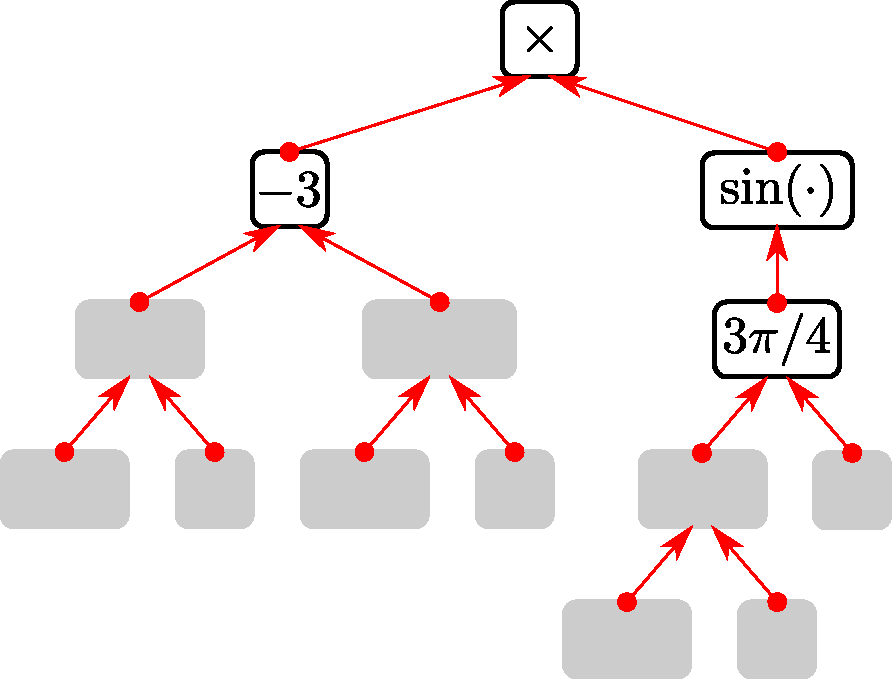
\includegraphics[width=55mm]{tree2c}
  & $\mapsto$
  & 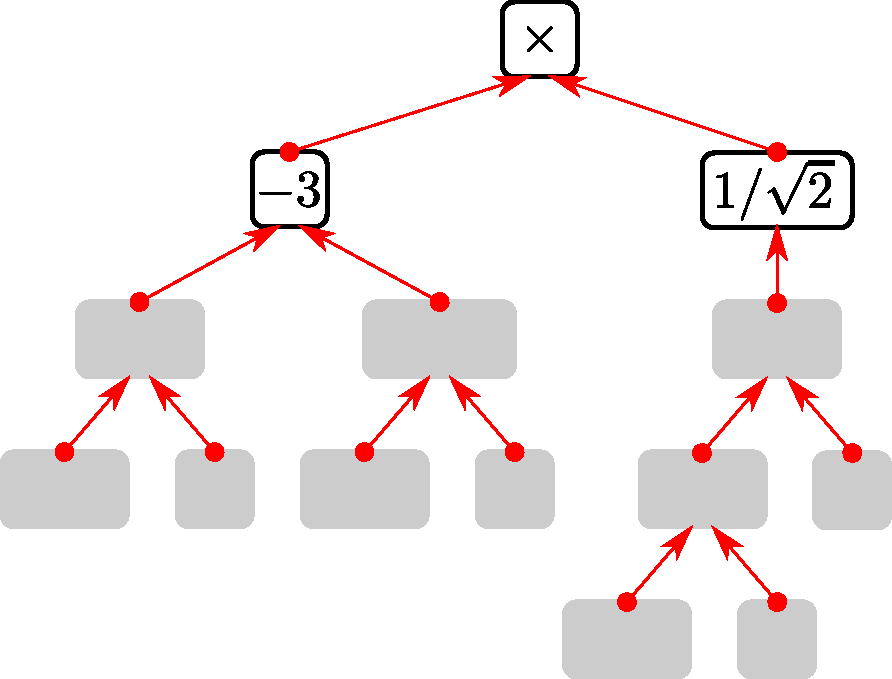
\includegraphics[width=55mm]{tree2d}
  & \\[15ex]
  $\mapsto$
  & 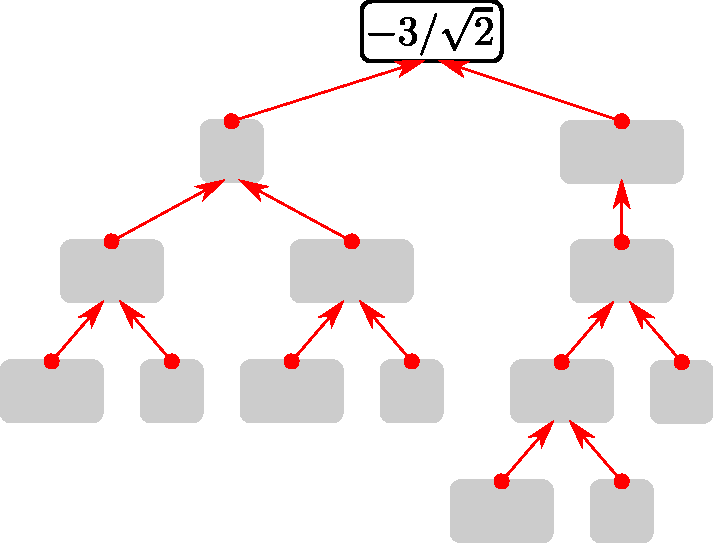
\includegraphics[width=55mm]{tree2e}
  & & and we are done.
\end{tabular}
\end{center}
\end{wfig}

\end{eg}

% \begin{eg}
%  And another one\dots
% \begin{align*}
%   \text{We need another nice example in here.}
% \end{align*}
% \end{eg}

It is highly unlikely that you will ever need to explicitly construct such a
tree for any problem in the remainder of the text. The main point of
introducing these objects and working through a few examples is to realise that
all the functions that we will examine are constructed from simpler pieces. In
particular we have constructed all the above examples from simple ``building
blocks''
\begin{itemize}
 \item constants --- fixed numbers like $1, \pi$ and so forth
 \item variables --- usually $x$ or $t$, but sometimes other symbols
 \item standard functions --- like trigonometric functions (sine, cosine and
tangent), exponentials and logarithms.
\end{itemize}
These simple building blocks are combined using arithmetic
\begin{itemize}
 \item addition and subtraction --- $a + b$ and $a-b$
\item multiplication and division --- $a \cdot b$ and $\nicefrac{a}{b}$
\item raising to a power --- $a^n$
\item composition --- given two functions $f(x)$ and $g(x)$ we form a
new function $f(g(x))$ by evaluating $y=g(x)$ and then evaluating $f(y) =
f(g(x))$.
\end{itemize}
During the rest of the course when we learn how to compute limits and
derivatives, our computations require us to understand the way we construct
functions as we have just described.

That is, in order to compute the derivative\footnote{We get to this in Chapter~\ref{chap
deriv} --- don't worry about exactly what it is just now.} of a function we
have to see how to construct the function from these building blocks (i.e. the
constants, variables and standard functions) using arithmetic operations. We
will then construct the derivative by following these same steps. There will be
simple rules for finding the derivatives of the simpler pieces and then rules
for putting them together following the arithmetic used to construct the function.


\section{Inverse Functions}\label{sec inverse functions}
There is one last thing that we should review before we get into the main material of the
course and that is inverse functions. As we have seen above functions are really just
rules for taking an input (almost always a number), processing it somehow (usually by a
formula) and then returning an output (again, almost always a number).
\begin{align*}
 \text{input number $x$} \quad \mapsto \quad \text{$f$ does ``stuff'' to $x$} \quad
\mapsto \quad \text{return number $y$}
\end{align*}
In many situations it will turn out to be very useful if we can undo whatever it is that
our function has done. ie
\begin{align*}
 \text{take output $y$} \quad \mapsto \quad \text{do ``stuff'' to $y$}
  \quad \mapsto \quad \text{return the original $x$}
\end{align*}
When it exists, the function ``which undoes'' the function $f(x)$ is found by solving
$y=f(x)$ for $x$ as a function of $y$ and is called the inverse function of $f$.
It turns out that it is not always possible to solve $y=f(x)$ for $x$ as a
function of $y$. Even when it is possible, it can be really hard to
do\footnote{Indeed much of encryption exploits the fact that you can find
functions that are very quick to do, but very hard to undo. For example --- it
is very fast to multiply two large prime numbers together, but very hard to take
that result and factor it back into the original two primes. The interested
reader should look up trapdoor functions.}.


For example --- a particle's position, $s$, at time $t$ is given by the formula
$s(t) = 7t$ (sketched below). Given a calculator, and any particular number $t$,
you can quickly work out the corresponding positions $s$. However, if you are
asked the question ``When does the particle reach $s=4$?'' then to answer it we
need to be able to ``undo'' $s(t)=4$ to isolate $t$. In this case, because
$s(t)$ is always increasing, we can always undo $s(t)$ to get a unique answer:
\begin{align*}
  s(t) &= 7t = 4 & \text{ if and only if }&& t&= \frac{4}{7}.
\end{align*}

However, this question is not always so easy. Consider the sketch of $y=\sin(x)$
below; when is $y=\half$? That is, for which values $x$ is $\sin(x)=\half$? To
rephrase it again, at which values of $x$ does the curve $y=\sin x$ (which is
sketched in the right
half of Figure~\ref{fig inv1}) cross the horizontal straight line $y=\frac{1}{2}$ (which
is also sketched in the same figure)?
\begin{fig}\label{fig inv1}
\begin{center}
 \includegraphics[height=5cm]{inv1}
\end{center}
\end{fig}
We can see that there are going to be an infinite number of $x$-values that give
$y=\sin(x)=\half$; there is no unique answer.

Recall (from Definition~\ref{def function}) that for any given input, a function must
give a unique output. So if we want to find a \emph{function} that undoes $s(t)$, then
things are good --- because each $s$-value corresponds to a unique $t$-value. On the
other hand, the situation with $y=\sin x$ is problematic --- any given $y$-value is
mapped to by many different $x$-values. So when we look for an \emph{unique} answer to
the question ``When is $\sin x = \half$?'' we cannot answer it.

This ``uniqueness'' condition can be made more precise:
\begin{defn}
 A function $f$ is one-to-one (injective) when it never takes the same $y$
value more than once. That is
\begin{align*}
  \mbox{if } x_1 \neq x_2 \mbox{ then } f(x_1) \neq f(x_2)
\end{align*}
\end{defn}
There is an easy way to test this when you have a plot of the function --- the
horizontal line test.
\begin{defn}[Horizontal line test]
 A function is one-to-one if and only if no horizontal line $y=c$ intersects
the graph $y=f(x)$ more than once.
\end{defn}
\noindent i.e. every horizontal line intersects the graph either zero or
one times. Never twice or more. This test tell us that $y=x^3$ is
one-to-one, but $y=x^2$ is not. However note that if we restrict the domain of
$y=x^2$ to $x \geq 0$ then the horizontal line test is passed. This is one of
the reasons we have to be careful to consider the domain of the function.
\begin{fig}
\begin{center}
 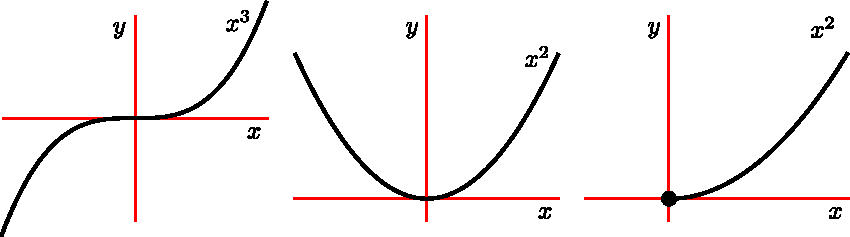
\includegraphics[height=3.5cm]{inv1A}
\end{center}
\end{fig}

When a function is one-to-one then it has an inverse function.
\begin{defn}\label{def inv func}
 Let $f$ be a one-to-one function with domain $A$ and range $B$. Then its inverse
function is denoted $f^{-1}$ and has domain $B$ and range $A$. It is defined by
\begin{align*}
  f^{-1}(y) &= x & \text{ whenever }&& f(x)&=y
\end{align*}
for any $y \in B$.
\begin{efig}
\begin{center}
 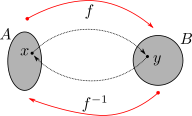
\includegraphics[height=4cm]{inv2}
\end{center}
\end{efig}
\end{defn}
So if $f$ maps $x$ to $y$, then $f^{-1}$ maps $y$ back to $x$. That is $f^{-1}$ ``undoes''
$f$. Because of this we have
\begin{align*}
  f^{-1}( f(x) ) &= x  &\mbox{ for any $x \in A$}\\
   f( f^{-1}(y) )&=y &\mbox{ for any $y \in B$}
\end{align*}
We have to be careful not to confuse $f^{-1}(x)$ with $\ds \frac{1}{f(x)}$. The ``$-1$''
is not an exponent.

\begin{eg}
Let $f(x)=x^5+3$ on domain $\mathbb{R}$. To find its inverse we do the following
\begin{itemize}
 \item Write $y=f(x)$; that is $y=x^5+3$.
 \item Solve for $x$ in terms of $y$ (this is not always easy) --- $x^5=y-3$, so
$x=(y-3)^{1/5}$.
\item The solution is $f^{-1}(y) = (y-3)^{1/5}$.
\item Recall that the ``$y$'' in $f^{-1}(y)$ is a dummy variable. That is,
$f^{-1}(y) = (y-3)^{1/5}$ means that if you feed the number $y$ into the function
$f^{-1}$ it outputs the number $(y-3)^{1/5}$. You may call the input variable anything
you like. So if you wish to call the input variable ``$x$'' instead of ``$y$'' then just
replace every $y$ in $f^{-1}(y)$ with an $x$.
\item That is $f^{-1}(x) = (x-3)^{1/5}$.
%  \item Then interchange $x \leftrightarrow y$ to get $f^{-1}(x)=y=(x-3)^{1/5}$.
\end{itemize}
\end{eg}


\begin{eg}
Let $g(x) = \sqrt{x-1}$ on the domain $x \geq 1$. We can find the inverse in the same way:
\begin{align*}
  y &= \sqrt{x-1} \\
  y^2 &= x-1 \\
  x &= y^2+1 = f^{-1}(y) & \text{or, writing input variable as ``$x$'':} \\
  f^{-1}(x) &= x^2+1.
\end{align*}
\end{eg}

Let us now turn to finding the inverse of $\sin(x)$ --- it is a little more tricky and we
have to think carefully about domains.


\begin{eg}
We have seen (back in Figure~\ref{fig inv1}) that $\sin(x)$ takes each value $y$
between $-1$ and $+1$ for infinitely many different values of $x$ (see
the left-hand graph in the figure below). Consequently $\sin(x)$, with domain
$-\infty <x <\infty$ does not have an inverse function.
\begin{wfig}
\begin{center}
 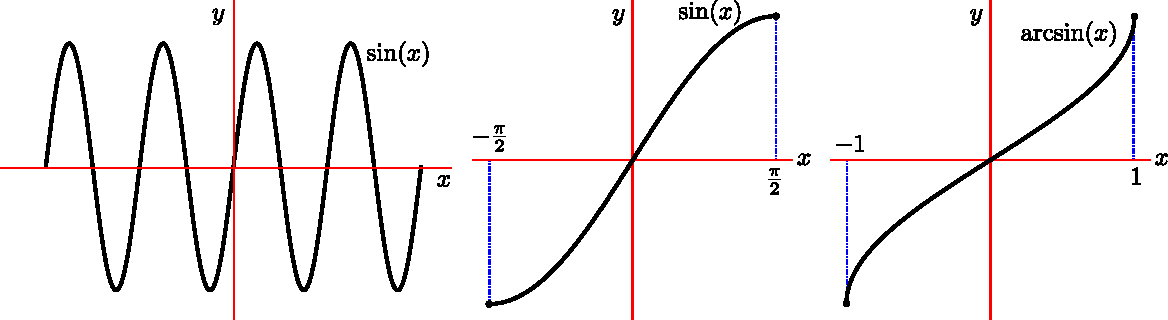
\includegraphics[height=4cm]{inv2B}
\end{center}
\end{wfig}
But notice that as $x$ runs from $-\frac{\pi}{2}$ to $+\frac{\pi}{2}$, $\sin(x)$ increases
from $-1$ to $+1$. (See the middle graph in the figure above.) In particular, $\sin(x)$
takes each value $-1 \le y\le 1$ for exactly one $-\frac{\pi}{2}\le x\le \frac{\pi}{2}$.
So if we restrict $\sin x$ to have domain $-\frac{\pi}{2}\le x\le \frac{\pi}{2}$, it does
have an inverse function, which is traditionally called arcsine (see Appendix~\ref{sec
inv trig}).

That is, by definition, for each $-1\le y\le 1$, $\arcsin(y)$ is the unique
$-\frac{\pi}{2}\le x\le \frac{\pi}{2}$ obeying $\sin(x)=y$. Equivalently, exchanging the
dummy variables x and y throughout the last sentence gives that for each $-1\le
x\le 1$, $\arcsin(x)$ is the unique $-\frac{\pi}{2}\le y\le \frac{\pi}{2}$
obeying $\sin(y)=x$.
\end{eg}



It is an easy matter to construct the graph of an inverse function
from the graph of the original function. We just need to remember that
\begin{equation*}
Y=f^{-1}(X)  \iff f(Y)=X
\end{equation*}
which is $y=f(x)$ with $x$ renamed to $Y$ and $y$ renamed to $X$.
%Each point on the graph of $f$ has coordinates $\big(x\,,\,f(x)\big)$.
%If we rename $x$ to $Y$, those coordinates become
%\begin{equation*}
%\big(Y,f(Y)\big) = \big(f^{-1}(X),X\big) = (Y,X)\quad\text{with}\quad Y=f^{-1}(X)
%\end{equation*}
%To get the graph of $f^{-1}$ we just need to reinterpret these statements
%graphically.

 Start by drawing the graph of $f$, labelling the $x$-- and $y$--axes
and labelling the curve $y=f(x)$.
\begin{efig}
\begin{center}
   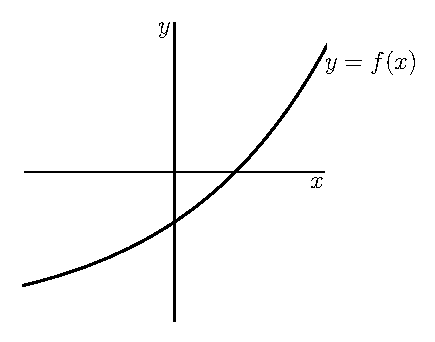
\includegraphics{fInvA}
\end{center}
\end{efig}
Now replace each $x$ by $Y$ and each $y$ by $X$  and replace the resulting
label $X=f(Y)$ on the curve by the equivalent $Y=f^{-1}(X)$.
\begin{efig}
\begin{center}
   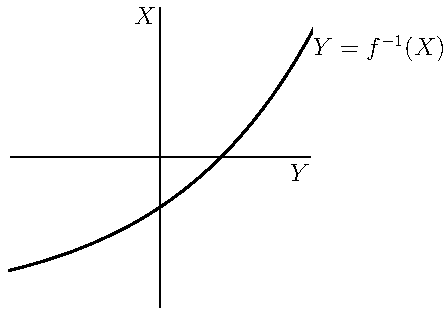
\includegraphics{fInvB}
\end{center}
\end{efig}
Finally we just need to redraw the sketch with the $Y$ axis running vertically
(with $Y$ increasing upwards) and the $X$ axis running horizontally (with
$X$ increasing to the right). To do so, pretend that the sketch is on
a transparency or on a very thin piece of paper that you can see through.
Lift the sketch up and flip it over so that the $Y$ axis runs vertically
and the $X$ axis runs horizontally. If you want, you can also convert the upper
case $X$ into a lower case $x$ and the upper case $Y$ into a lower case
$y$.
\begin{wfig}
\begin{center}
   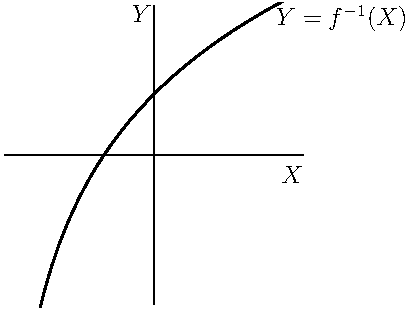
\includegraphics{fInvC}\qquad   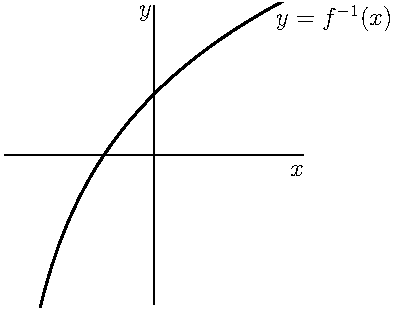
\includegraphics{fInvD}
\end{center}
\end{wfig}
Another way to say ``flip the sketch over so as to exchange the
$x$-- and $y$--axes'' is ``reflect in the line $y=x$''. In the
figure below the blue ``horizontal'' elliptical disk that is centred
on $(a,b)$ has been reflected in the line $y=x$ to give the red ``vertical''
elliptical disk centred on $(b,a)$.
\begin{wfig}
\begin{center}
   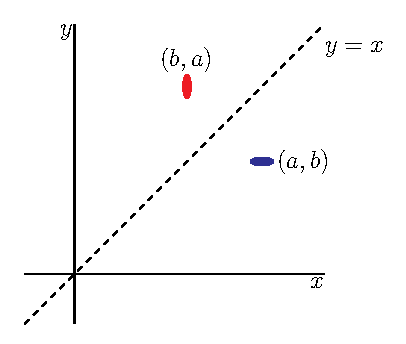
\includegraphics{fInvR}
\end{center}
\end{wfig}

\begin{eg}\label{eg:INVlogbaseten}
As an example, let $f(x) = x^2$ with domain $0\le x< \infty$.
\begin{itemize}\itemsep1pt \parskip0pt \parsep0pt \itemindent 10pt
\item
When $x=0$, $f(x)=0^2=0$.
\item
As $x$ increases, $x^2$ gets bigger and bigger.
\item
When $x$ is very large and positive,
$x^2$ is also very large and positive.
(For example, think $x=100$.)
\end{itemize}
The graph of $y=f(x)=x^2$ is the blue curve below.
By definition, $Y=f^{-1}(X)$ if $X=f(Y)=Y^2$. That is, if $Y=\sqrt{X}$.
(Remember that, to be in the domain of $f$, we must have $Y\ge 0$.)
So the inverse function of ``square'' is ``square root''. The
graph of $f^{-1}$ is the red curve below. The red curve is the
reflection of the blue curve in the line $y=x$.
\begin{wfig}
\begin{center}
   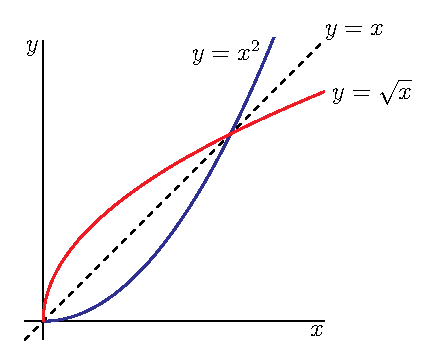
\includegraphics{fInvSqA}
\end{center}
\end{wfig}
\end{eg}
